\documentclass[14pt,aspectratio=169]{beamer}
\usepackage[utf8]{inputenc}
\usepackage[spanish]{babel}
\usepackage{xcolor}
%\usepackage{biblatex}
%\addbibresource{presentacion.bib}
%\setbeamertemplate{bibliography item}{\insertbiblabel}
\usepackage[autostyle=true]{csquotes}

\usetheme{Copenhagen}
%\setbeamercolor{background canvas}{bg=white}
\definecolor{verde}{rgb}{.25,.5,.25}
\usecolortheme[named=verde]{structure}

\usepackage{helvet}

\title{Edición ramificada}
\subtitle{La edición por venir}
\author{Alberto Moyano}
\date{14 de mayo de 2024}
\institute{\url{https://gitlab.com/alberto.alejandro.moyano/CHARLAMATE}}

\setbeamertemplate{headline}{}
\setbeamertemplate{navigation symbols}{}
\setbeamercovered{transparent}

\begin{document}

	\begin{frame}
		\titlepage
	\end{frame}

\begin{frame}{Un poco de historia}
	¿Cómo es la edición que conocemos?

	\begin{figure}
	\centering
	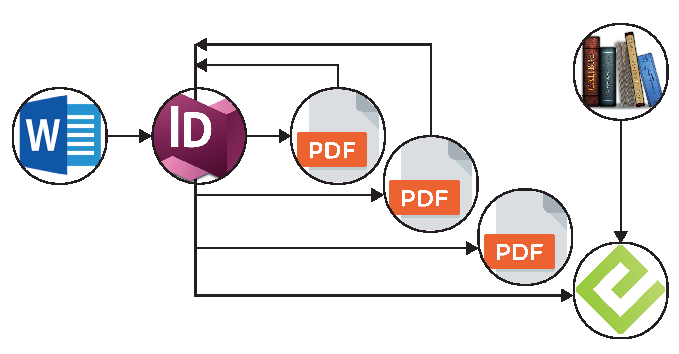
\includegraphics[width=.7\textwidth]{ciclos.pdf}
\end{figure}
\end{frame}

\begin{frame}{Un poco de historia}
	La edición de libros y revistas en tiempos preinformáticos
	\begin{figure}
		\centering
		\includegraphics[width=.7\textwidth]{gutenberg.pdf}
	\end{figure}
\end{frame}

\begin{frame}{Un solo origen}
	¿Qué es la edición ramificada en el campo editorial?\vspace{14pt}

	\begin{quote}
	Refiere a un modelo de producción a partir de un único origen, en donde se configuran salidas independientes para diferentes necesidades o requisitos sin afectar el contenido del origen principal.
	\end{quote}
\end{frame}

\begin{frame}{Editoriales y modelos en juego}
	\begin{enumerate}
		\item \url{https://www.oreilly.com/} (asciidoc y LaTeX)
		\item \url{https://brill.com/} (le-tex)
		\item \url{https://www.elsevier.com/es-es} (le-tex)
		\item \url{https://www.le-tex.de/en/} (LaTeX)
		\item \url{https://www.softcover.io/} (markdown y LaTeX)
		\item \url{gbtexpublisher/} (LaTeX)
	\end{enumerate}
\end{frame}

\begin{frame}{Lenguajes de marcas}
	\begin{enumerate}
		\item Markdown: marcado ligero diseñado para ser fácil de leer y escribir, con una sintaxis básica.\\
		\url{https://daringfireball.net/projects/markdown/}
		\item AsciiDoc: marcado diseñado para ser fácil de leer y escribir, con una sintaxis simple y legible.\\
		\url{https://asciidoc.org/}
		\item LaTeX: sistema de preparación de documentos, se utiliza para la creación de documentos científicos.\\
		\url{https://www.latex-project.org/}
	\end{enumerate}
\end{frame}

\begin{frame}{Modelo estrella}
	\begin{figure}
		\centering
		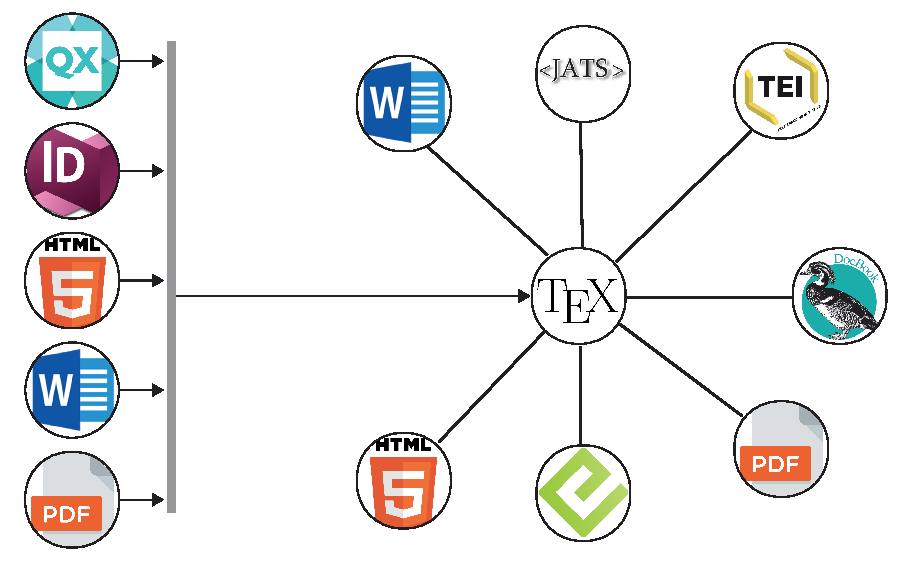
\includegraphics[width=.7\textwidth]{estrella.pdf}
	\end{figure}
\end{frame}

\begin{frame}{Modelo árbol}
	\begin{figure}
		\centering
		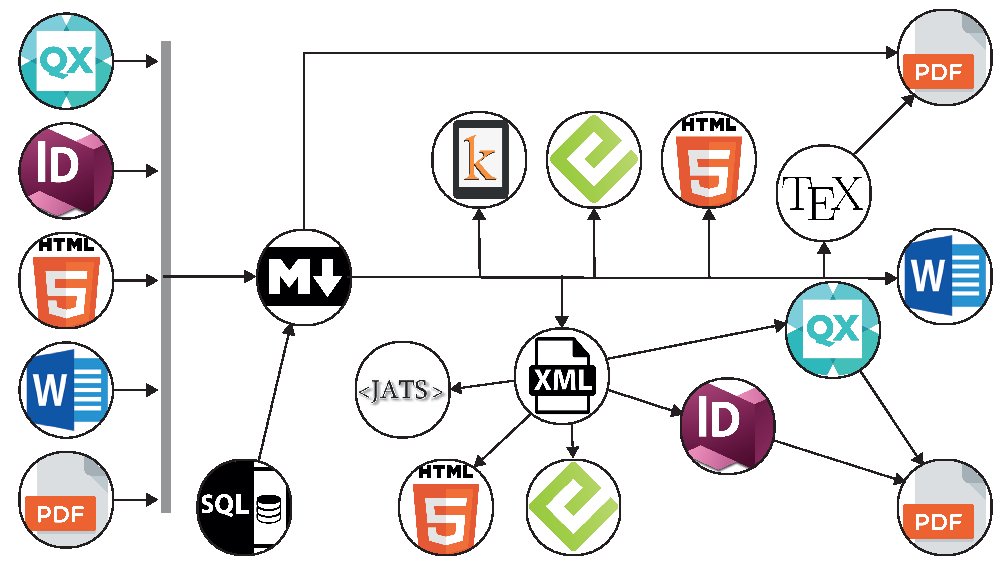
\includegraphics[width=.8\textwidth]{completo.pdf}
	\end{figure}
\end{frame}

\begin{frame}{Modelo árbol}
	\begin{figure}
		\centering
		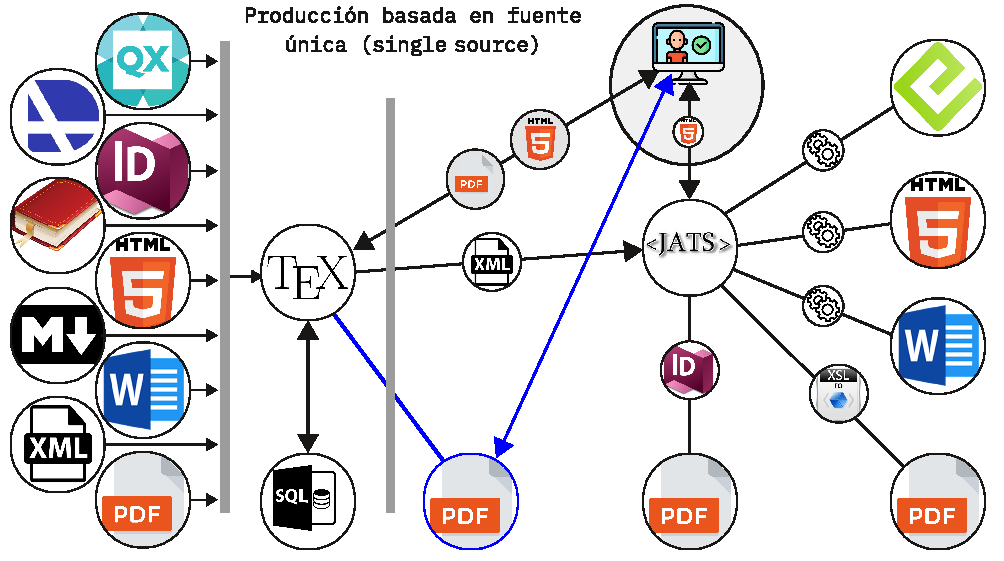
\includegraphics[width=.8\textwidth]{arbol2.pdf}
	\end{figure}
\end{frame}

\begin{frame}{Modelo árbol}
	\begin{figure}
		\centering
		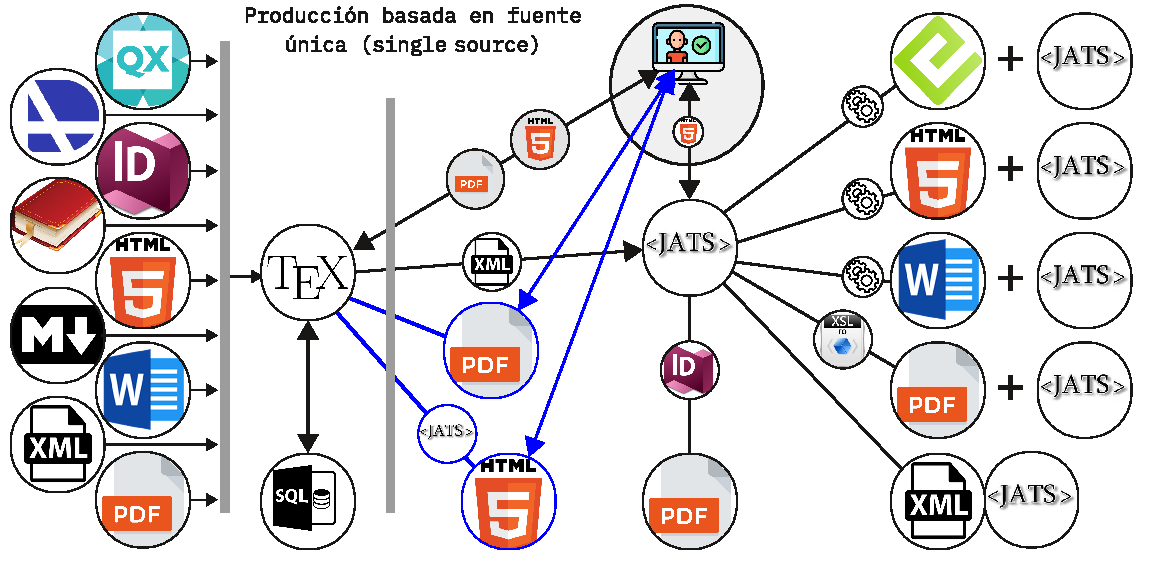
\includegraphics[width=.9\textwidth]{arbol3.pdf}
	\end{figure}
\end{frame}

\begin{frame}[allowframebreaks]{La edición ramificada}
Está diseñada para avanzar en un flujo de producción editorial flexible y multisoporte. Algunas ventajas que se pueden observar:

\begin{itemize}
\item \textbf{Facilidad de trabajo:} permite a los editores trabajar en nuevas características o correcciones de errores sin afectar la rama principal.% Esto significa que se puede experimentar sin preocuparse por romper la versión estable del libro o revista.
\item \textbf{Mejora en la colaboración:} varias personas pueden trabajar en diferentes ramas simultáneamente, lo que facilita la colaboración en editoriales grandes o distribuidas.% Cada sector puede concentrarse en su tarea sin interferir con el trabajo de los demás hasta que esté listo para fusionarse con la rama principal.
\item \textbf{Gestión de versiones estables:} las ramas permiten mantener versiones estables del libro o revista mientras continúa la edición en otras ramas.
\item \textbf{Experimentación controlada:} las ramas proporcionan un entorno aislado para experimentar con nuevas ideas o cambios radicales en la representación de los datos.% Si una idea no funciona como se esperaba, se puede descartar sin afectar la rama principal del proyecto.
\item \textbf{Facilidad para revertir cambios:} si un cambio introducido en una rama resulta ser problemático o no deseado, es relativamente fácil revertir esos cambios sin afectar otras partes del proyecto.% Esto ayuda a mantener la estabilidad y facilita la resolución de problemas.
\end{itemize}
\end{frame}

\begin{frame}{Gracias}
	Agradezco a los presentes la oportunidad de poder difundir estas ideas, para quienes me quieran contactar, dejo mis datos.
\begin{itemize}
	\item Alberto Moyano
	\item +54 11 6113.0328
	\item alberto.alejandro.moyano@gmail.com
	\item \url{https://github.com/albertomoyano/}
	\item \url{https://www.linkedin.com/in/edicion-cientifica/}
\end{itemize}
\end{frame}

%\nocite{*}
%\begin{frame}{Para saber más}
%	\printbibliography
%\end{frame}

\end{document}
